% partes/parte1/cap03.tex
\chapter{Gestión de datos del consumidor: valor, omnicanalidad, escucha y decisión}
\label{cap:03}

\begin{cajaFicha}
\begin{description}
  \item[Unidad temática] I — Comportamiento, perfil y gestión de datos del consumidor digital.
  \item[Temas del programa] 1.3 Gestión de datos de los consumidores digitales: 1.3.1 Creación de valor para el consumidor-usuario (CX-UX); 1.3.2 Experiencias omnicanal consumidor-usuario (CX-UX); 1.3.3 Momentos de escucha a los consumidores digitales; 1.3.4 Importancia de la recolección y gestión de datos; 1.3.5 Toma de decisiones basadas en la gestión de datos digitales.
  \item[Horas] Teoría 2.0 · Práctica 5.0 · Aprendizaje autónomo 2.0.
  \item[Competencia de la unidad] Identifica el comportamiento del consumidor digital y su evolución a partir de sus tipos de perfil y gestión de datos.
  \item[Resultados de aprendizaje observables] Al concluir el capítulo, el estudiante:
  \begin{enumerate}
    \item distingue experiencia de cliente (CX) de experiencia de usuario (UX) y las ubica en el mapa de gestión de datos;
    \item aplica limpieza de datos, segmentación RFM y una prueba A/B para fundamentar una decisión;
    \item explica el marco legal mexicano vigente de protección de datos personales y sus implicaciones para la recolección de datos del consumidor.
  \end{enumerate}
  \item[Prerrequisitos] Cap. 1--2.
\end{description}
\end{cajaFicha}

\section{Caso de apertura}

Una cadena de farmacias mexicana descubre, al revisar sus datos de
fidelidad, que el 60\,\% de las personas que abandonan su carrito de compra
en la app lo hacen en el mismo paso: la solicitud de un segundo número
telefónico para verificación en dos pasos. Nadie diseñó ese paso para
espantar clientes. Se agregó por seguridad, se probó internamente, funcionó
bien. El dato de abandono —que solo existe porque la organización recolecta
y analiza sistemáticamente el comportamiento en su app— es lo que revela un
problema invisible al ojo humano. Este capítulo trata sobre esa cadena
completa: cómo se recolectan los datos, qué los vuelve confiables, cómo se
escucha al consumidor a través de ellos, y qué obligaciones legales trae
consigo tenerlos.

\section{Desarrollo teórico}

\begin{figure}[htbp]
  \centering
  \resizebox{\textwidth}{!}{% figuras/tikz/cap03-mapa-gestion-datos.tex
% Mapa de gestión de datos del consumidor digital: recolección -> decisión.
% Pieza de Parte I requerida por §10 del prompt de proyecto.
\begin{tikzpicture}[
    etapa/.style={rectangle, rounded corners, draw=guindaIPN, thick, fill=guindaIPNClara,
                  minimum width=2.5cm, minimum height=1.3cm, align=center, font=\scriptsize},
    flecha/.style={-{Stealth[length=2.8mm]}, thick, draw=doradoIPN}
  ]
  \node[etapa] (rec) at (0,0)    {Recolección\\ (§1.3.4)};
  \node[etapa] (lim) at (3,0)    {Limpieza y\\ calidad};
  \node[etapa] (esc) at (6,0)    {Escucha\\ (§1.3.3)};
  \node[etapa] (val) at (9,0)    {Creación\\ de valor\\ CX-UX (§1.3.1)};
  \node[etapa] (dec) at (12,0)   {Decisión\\ (§1.3.5)};

  \draw[flecha] (rec) -- (lim);
  \draw[flecha] (lim) -- (esc);
  \draw[flecha] (esc) -- (val);
  \draw[flecha] (val) -- (dec);

  \node[etapa, fill=terracotaIPNClara, draw=terracotaIPN, minimum width=11.5cm, minimum height=0.9cm]
    (base) at (5.5,-2) {Base legal y consentimiento (LFPDPPP) — condición de todo el mapa, no un paso más};
  \draw[flecha] (base.north -| rec) -- (rec.south);
  \draw[flecha] (base.north -| dec) -- (dec.south);
\end{tikzpicture}
}
  \caption{Mapa de gestión de datos del consumidor digital: de la
  recolección a la decisión, con la base legal como condición transversal, no
  como un paso más de la cadena. Fuente: elaboración propia.}
  \label{fig:cap03-mapa}
\end{figure}

\subsection{Creación de valor para el consumidor-usuario (CX-UX)}
\progtag{1.3.1}

CX (\textit{customer experience}, experiencia de cliente) y UX
(\textit{user experience}, experiencia de usuario) no son sinónimos, aunque
el capítulo del programa oficial las agrupe bajo una misma sigla compuesta y
buena parte de la bibliografía de comportamiento del consumidor las trate
como intercambiables \parencite{hoyer2024consumer}.
UX es el diseño de la interacción con un producto o interfaz específicos
—qué tan fácil es completar una tarea en una app—. CX es la suma de todas
las interacciones de una persona con una organización a lo largo del tiempo
y de los canales —de las cuales UX es una parte, no el todo—. Una app puede
tener una UX impecable (fácil de usar, rápida) dentro de una CX deficiente
(si, por ejemplo, el servicio al cliente detrás de esa app es lento o
inconsistente). Distinguir ambas evita el error común de optimizar la
interfaz mientras el resto de la relación con el cliente se deteriora sin
que ningún panel de control lo esté midiendo.

\subsection{Experiencias omnicanal consumidor-usuario (CX-UX)}
\progtag{1.3.2}

La definición académica de referencia es la de Verhoef, Kannan e Inman:
omnicanalidad es \enquote{la gestión sinérgica de los múltiples canales y
puntos de contacto disponibles, de forma que la experiencia del cliente a
través de los canales y el desempeño a través de los canales se optimicen}
\parencite{verhoef2015}. La palabra clave es \textit{sinérgica}: no basta con
que una organización esté presente en varios canales (multicanalidad); la
omnicanalidad exige que esos canales compartan una sola identidad de cliente
reconocible (figura~\ref{fig:cap03-omnicanal}), de modo que un consumidor que
empieza una compra en la app y la termina en tienda física sea tratado como
la misma persona, no como dos registros distintos.

\begin{figure}[htbp]
  \centering
  % figuras/tikz/cap03-omnicanal.tex
% Experiencias omnicanal: puntos de contacto distintos que deben resolver a
% una sola identidad de cliente (Verhoef, Kannan & Inman, 2015).
\begin{tikzpicture}[
    canal/.style={rectangle, rounded corners, draw=bronceIPN, thick, fill=bronceIPNClaro,
                  minimum width=2.4cm, minimum height=0.9cm, align=center, font=\scriptsize},
    centro/.style={circle, draw=guindaIPN, very thick, fill=guindaIPNClara,
                   minimum size=2.4cm, align=center, font=\small},
    flecha/.style={-{Stealth[length=2.5mm]}, thick, draw=doradoIPN}
  ]
  \node[centro] (id) at (0,0) {Identidad\\ única de\\ cliente};

  \node[canal] (app)    at (-4.2, 2.2) {App móvil};
  \node[canal] (web)    at (0, 3.2)    {Sitio web};
  \node[canal] (tienda) at (4.2, 2.2)  {Tienda física};
  \node[canal] (social) at (-4.2,-2.2) {Redes sociales};
  \node[canal] (cc)     at (4.2,-2.2)  {Centro de contacto};

  \foreach \n in {app,web,tienda,social,cc} {
    \draw[flecha] (\n) -- (id);
  }
\end{tikzpicture}

  \caption{Experiencia omnicanal: puntos de contacto distintos que deben
  resolver a una sola identidad de cliente. Fuente: elaboración propia con
  base en \parencite{verhoef2015}.}
  \label{fig:cap03-omnicanal}
\end{figure}

Resolver esa identidad única es, en la práctica, un problema técnico difícil
—el mismo problema que atraviesa el fin de las cookies de terceros y el giro
a datos de primera parte que se discute en el recuadro de Frontera de este
capítulo—, y también un problema legal: unificar el rastro de una persona
entre canales es, por definición, tratamiento de datos personales, sujeto a
la ley que se revisa en la §2.4.

\subsection{Momentos de escucha a los consumidores digitales}
\progtag{1.3.3}

\enquote{Escuchar} a un consumidor digital no significa, la mayor parte del
tiempo, leer lo que escribe. Significa observar tres tipos de señal
distintos: la señal declarada (lo que el consumidor dice explícitamente —una
reseña, una encuesta, un comentario en redes—), la señal conductual (lo que
el consumidor hace —qué compra, dónde se detiene, qué abandona—) y la señal
de contexto (las circunstancias en que ocurre la interacción —hora, canal,
dispositivo—). El caso de apertura de este capítulo es un ejemplo de escucha
puramente conductual: nadie tuvo que quejarse del segundo número telefónico
para que el problema fuera visible en los datos. Un programa de escucha que
solo atiende la señal declarada (encuestas de satisfacción, menciones en
redes) sistemáticamente subestima estos problemas silenciosos, porque la
mayoría de los consumidores que abandonan una compra no se queja: simplemente
se va.

\subsection{Importancia de la recolección y gestión de datos}
\progtag{1.3.4}

\begin{cajaFrontera}
\textbf{Datos de primera y de cero parte, y el mito del fin de las cookies de
terceros.} \enquote{Datos de primera parte} son los que una organización
recolecta directamente de su propia relación con el consumidor (compras,
registro, navegación en su propio sitio); \enquote{datos de cero parte} son los
que el consumidor entrega de forma voluntaria y explícita (una encuesta de
preferencias, un cuestionario de talla). Ambos ganaron relevancia
estratégica por presión regulatoria (la LFPDPPP que se revisa en la §2.4) y
por el supuesto fin de las cookies de terceros en los navegadores. Pero ese
supuesto fin no ocurrió como se anunció: Google revirtió en 2024 su plan de
depreciación de cookies de terceros en Chrome, descartó también el mecanismo
alternativo de \textit{choice prompt} en abril de 2025, y retiró las APIs de
reemplazo de Privacy Sandbox en octubre de 2025
\parencite{eprs2025darkpatterns}. \textbf{Vigente a septiembre de 2026:} las
cookies de terceros siguen activas por defecto en Chrome. El giro hacia
datos de primera y de cero parte sigue siendo la estrategia correcta —por
razones de confianza del consumidor y de cumplimiento legal, no solo
técnicas—, pero el capítulo advierte contra repetir la narrativa de
\enquote{las cookies ya desaparecieron}, que circula ampliamente en el
discurso de mercadotecnia digital sin corresponder a los hechos verificables
a la fecha de este libro.
\end{cajaFrontera}

El marco legal mexicano de protección de datos personales cambió de forma
sustancial en 2025. El cuadro~\ref{tab:cap03-lfpdppp} resume la cronología
verificada contra fuentes oficiales.

\begin{table}[htbp]
\centering
\begin{tabular}{@{}p{2.6cm}p{9.6cm}@{}}
\toprule
Fecha & Hecho jurídico \\
\midrule
20-dic-2024 & Reforma constitucional de simplificación orgánica: se decreta la desaparición del INAI, entre otros seis organismos autónomos \parencite{dof_simplificacion2024}. \\
20-mar-2025 & Se publica en el DOF la nueva Ley Federal de Protección de Datos Personales en Posesión de los Particulares (LFPDPPP), que abroga la ley de 2010; entra en vigor al día siguiente \parencite{dof_lfpdppp2025}. \\
9-may-2025 & Se formaliza la entrega-recepción institucional del INAI a la Secretaría Anticorrupción y Buen Gobierno, que asume las atribuciones de protección de datos personales de particulares \parencite{sabg2025entregarecepcion}. \\
14-nov-2025 & Reforma de homologación normativa a la LFPDPPP \parencite{dof_lfpdppp_reforma2025nov}. \\
\bottomrule
\end{tabular}
\caption{Cronología verificada de la reforma a la protección de datos
personales en México. Fuente: elaboración propia con base en el Diario
Oficial de la Federación y comunicados oficiales de gob.mx.}
\label{tab:cap03-lfpdppp}
\end{table}

Hay un punto de la nueva ley que este libro presenta con cautela deliberada,
en vez de con una postura firme: según fuentes de análisis jurídico
corporativo consultadas en la investigación de este libro, la nueva LFPDPPP
establecería el consentimiento tácito como regla general para el tratamiento
de datos personales —salvo datos sensibles—, mientras que, según esas mismas
fuentes, la ley también exigiría que el consentimiento sea libre, específico
e informado. Esta aparente tensión entre ambos principios no se resuelve en
este libro: se señala explícitamente para que el estudiante sepa que existe,
y se recomienda consultar el texto vigente de la ley y, para una decisión
profesional real, a un especialista en derecho de protección de datos antes
de diseñar un mecanismo de consentimiento con implicaciones legales.

\subsection{Toma de decisiones basadas en gestión de datos digitales}
\progtag{1.3.5}

La mercadotecnia impulsada por datos (\textit{data-driven marketing}) es uno
de los ejes centrales de la lectura contemporánea del marketing digital
\parencite{kotler2021marketing50}. Un dato limpio, bien recolectado y con
base legal es una condición necesaria para decidir bien; no es, por sí sola,
condición suficiente. Hace
falta, además, un método que traduzca el dato en decisión sin engañarse a
sí mismo por diseño. El laboratorio de este capítulo desarrolla tres de esos
métodos, en orden creciente de exigencia: limpiar datos antes de usarlos,
segmentar clientes por valor con RFM, y —el más exigente de los tres— probar
una decisión con un experimento controlado (A/B) en vez de decidir por
intuición o por la primera diferencia que se observe en un panel.

\section{Evidencia de México y del mundo}

\begin{table}[htbp]
\centering
\begin{tabular}{@{}lr@{}}
\toprule
Indicador (2024) & Cifra \\
\midrule
Personas con al menos un producto financiero formal & 76.5\,\% \\
Brecha de género en tenencia de producto financiero & 72.8\,\% mujeres vs. 80.9\,\% hombres \\
Personas que llevan registro de sus gastos o los de su hogar & 65.3\,\% \\
\bottomrule
\end{tabular}
\caption{Indicadores de gestión de información financiera personal en
México. Fuente: elaboración propia con datos de INEGI/CNBV, Encuesta
Nacional de Inclusión Financiera (ENIF) 2024, Comunicado de prensa 49/25
\parencite{inegi2025enif}.}
\label{tab:cap03-enif}
\end{table}

El dato de la brecha de género en el cuadro~\ref{tab:cap03-enif} —ocho
puntos porcentuales— es relevante para este capítulo más allá de su interés
demográfico: cualquier organización que segmente por comportamiento
financiero sin ponderar esta brecha corre el riesgo de que su definición de
\enquote{cliente de alto valor} termine, sin proponérselo, subrepresentando a
las mujeres del mercado que analiza —un ejemplo concreto de cómo una decisión
técnica de segmentación (§2 del Cap. 2) puede heredar un sesgo social ya
presente en los datos de origen, sin que ningún paso del proceso lo haga
explícito. La brecha se enmarca, además, en un crecimiento general de la
conectividad mexicana —86.1\,\% de la población de 6 años o más ya usa
internet en 2025 \parencite{inegi2026endutih}— que hace cada vez más costoso,
en términos de mercado potencial no capturado, ignorar sesgos de este tipo
en el diseño de un sistema de gestión de datos.

\section{Laboratorio MATLAB: RFM, CLV y prueba A/B}

\begin{cajaLaboratorio}
\textbf{Objetivo.} Limpiar un conjunto de datos transaccionales con valores
faltantes y atípicos, segmentar clientes por valor con el método RFM
(Recencia, Frecuencia, Monto), calcular un valor de vida del cliente (CLV)
simple, y decidir entre dos versiones de una página de checkout con una
prueba A/B basada en un test estadístico, no en la simple comparación de
porcentajes.

\textbf{Concepto detrás del código.} RFM puntúa a cada cliente en tres
dimensiones (recencia: qué tan reciente fue su última compra; frecuencia:
cuántas compras hizo; monto: cuánto gastó en promedio), típicamente por
quintiles, y combina los tres puntajes en un segmento. El CLV simple usado
aquí es
\[
  \mathrm{CLV}_i = \text{monto}_i \times \text{frecuencia}_i \times \text{horizonte (años)},
\]
una aproximación didáctica —no incorpora tasa de descuento ni probabilidad
de retención, que un CLV de negocio real sí debería considerar—. La prueba
A/B compara dos proporciones (tasa de conversión de la versión A vs. B) con
un test $z$ de dos proporciones:
\[
  z = \frac{\hat{p}_B - \hat{p}_A}{\sqrt{\hat{p}(1-\hat{p})\left(\frac{1}{n_A}+\frac{1}{n_B}\right)}},
  \qquad \hat{p} = \frac{x_A + x_B}{n_A + n_B},
\]
donde $\hat{p}$ es la proporción conjunta bajo la hipótesis nula de que
ambas versiones convierten igual.

\textbf{Script.} \texttt{matlab/cap03/cap03\_rfm\_clv\_ab.m}. Es el
\textbf{mismo script, sin modificar}, que se usa en la Práctica 2 de esta
Parte. Corrida tal como está, usa 300 clientes \textbf{sintéticos}
(\texttt{rng(42)}), con 5\,\% de valores faltantes y 2\,\% de atípicos
introducidos a propósito para que el bloque de limpieza tenga un problema
real que resolver.

\begin{lstlisting}[style=MATLABStyle, caption={Bloque de parámetros editable (\texttt{cap03\_rfm\_clv\_ab.m}) — es lo único que cambia entre corridas.}]
nClientes = 300;    % tamano de la base sintetica (Bloques 1-2)
horizonteAnios = 3; % horizonte del CLV simple
alfa = 0.05;         % significancia de la prueba A/B (Bloque 3)
nA = 1200; conversionesA = 132;   % version A (control)
nB = 1180; conversionesB = 159;   % version B (variante)
\end{lstlisting}

\textbf{Salida esperada.} Dos figuras: distribución de segmentos RFM y CLV
promedio por segmento (figura~\ref{fig:cap03-rfmclv}), y resultado de la
prueba A/B con intervalos de confianza (figura~\ref{fig:cap03-ab}).

\begin{center}
  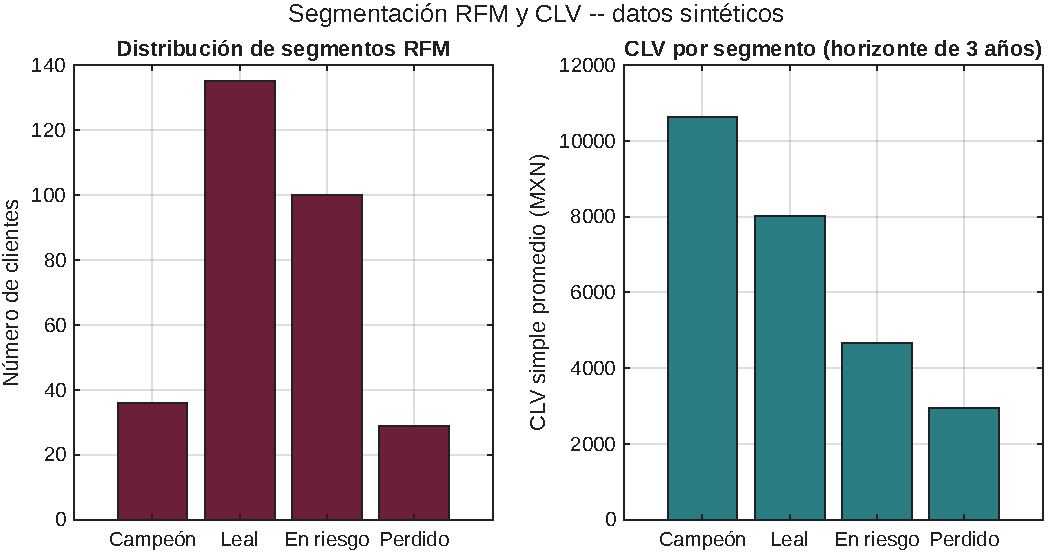
\includegraphics[width=0.98\textwidth]{figuras/matlab/cap03_rfm_clv.pdf}
  \captionof{figure}{Segmentación RFM (izquierda) y CLV simple promedio por
  segmento (derecha). Fuente: elaboración propia con datos sintéticos,
  \texttt{rng(42)}.}
  \label{fig:cap03-rfmclv}
\end{center}

\begin{center}
  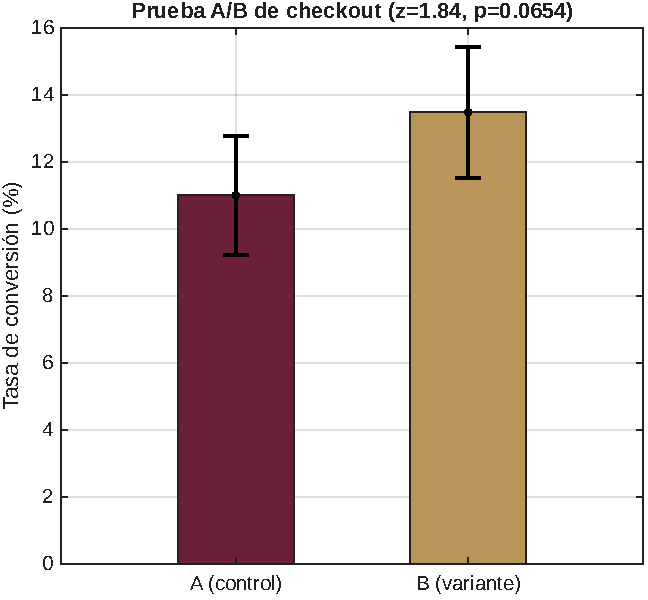
\includegraphics[width=0.62\textwidth]{figuras/matlab/cap03_prueba_ab.pdf}
  \captionof{figure}{Prueba A/B de checkout: la versión B convierte 2.5
  puntos porcentuales más, pero la diferencia no alcanza significancia
  estadística al 95\,\% ($p=0.065$). Fuente: elaboración propia con datos
  sintéticos.}
  \label{fig:cap03-ab}
\end{center}

\textbf{Interpretación de negocio.} El resultado de la prueba A/B es
deliberadamente el más instructivo del laboratorio: la versión B parece
mejor a simple vista (13.5\,\% contra 11.0\,\% de conversión), y un equipo
que decida \enquote{por el ojo} adoptaría B sin dudar —exactamente el tipo de
juicio bajo incertidumbre que Tversky y Kahneman documentan como propenso a
la heurística de representatividad, ver diferencia donde solo hay ruido
muestral \parencite{tverskykahneman1974}. El test estadístico
dice otra cosa: con $p=0.065$, apenas por encima del umbral convencional de
0.05, la diferencia observada es compatible con el azar. Los intervalos de
confianza de la figura~\ref{fig:cap03-ab} se traslapan de forma visible, lo
que confirma la misma conclusión sin necesidad de leer el valor $p$. La
decisión correcta no es \enquote{B es mejor, cámbiate} ni \enquote{no hay
diferencia, no importa}: es reconocer que la muestra actual no permite
concluir con la confianza convencional, y que la opción disciplinada es
correr la prueba más tiempo o con más tráfico antes de decidir —exactamente
el tipo de paciencia que la presión de negocio, en la práctica, más cuesta
sostener.

\textbf{Ejercicio propuesto (usen exactamente este script, solo cambien el
bloque de parámetros).} Corran el script tres veces y completen un cuadro
con la conversión de cada versión, el estadístico $z$, el valor $p$ y la
decisión que imprime cada corrida:
\begin{enumerate}
  \item \textbf{Caso A — valores por defecto:} $n_A=1200$, conversiones$_A=132$;
  $n_B=1180$, conversiones$_B=159$; $\alpha=0.05$.
  \item \textbf{Caso B — mismas tasas, más muestra:} multipliquen por 5 los
  cuatro valores de la prueba A/B ($n_A=6000$, conversiones$_A=660$;
  $n_B=5900$, conversiones$_B=795$), sin cambiar $\alpha$.
  \item \textbf{Caso C — mismos datos del Caso A, umbral más laxo:}
  regresen a los valores del Caso A y cambien solo $\alpha$ a 0.10.
\end{enumerate}
Con el cuadro completo, respondan por escrito: ¿cambia la decisión entre el
Caso A y el Caso B, aunque las proporciones observadas sean idénticas? ¿A
qué se debe? ¿Cambia la decisión entre el Caso A y el Caso C? ¿Qué tipo de
error (falso positivo o falso negativo) se vuelve más probable al relajar
$\alpha$, y en qué escenarios de negocio sería aceptable correr ese riesgo?

\textbf{Extensión opcional.} Incorporar una tasa de descuento al cálculo de
CLV (CLV descontado a valor presente) y comparar el orden resultante de los
cuatro segmentos contra el CLV simple del script.
\end{cajaLaboratorio}

\begin{cajaEtica}
La reforma a la LFPDPPP resumida en el cuadro~\ref{tab:cap03-lfpdppp} sigue
activa: hubo una reforma en noviembre de 2025 y es razonable esperar más
ajustes. Ninguna decisión de recolección de datos de este capítulo —ni la
resolución de identidad omnicanal, ni la segmentación RFM con datos reales,
ni ningún mecanismo de consentimiento— debe diseñarse a partir de lo que
diga este libro como fuente única. La responsabilidad profesional incluye
verificar el estado vigente de la ley al momento de implementar, no solo al
momento de estudiar.
\end{cajaEtica}

\section{Estudio de caso}

\begin{casoFicticio}
Una plataforma de cursos en línea nota que su tasa de finalización de
cursos gratuitos es del 8\,\%, y decide probar un rediseño del panel de
progreso del estudiante (barra de avance más visible, recordatorios por
correo). Corre una prueba A/B durante dos semanas con 400 estudiantes por
grupo: la versión con el rediseño muestra una finalización de 11\,\%, contra
8.5\,\% de la versión de control. El equipo de producto presenta el
resultado a la dirección como \enquote{el rediseño aumenta la finalización 3
puntos porcentuales, hay que lanzarlo a todos los usuarios}.

\textbf{Preguntas guía.}
\begin{enumerate}
  \item Con los datos dados (400 y 400 estudiantes, 11\,\% y 8.5\,\%),
  replique el cálculo del test $z$ de dos proporciones del laboratorio y
  determine si la diferencia es estadísticamente significativa al 95\,\%.
  \item Si el resultado no fuera significativo, ¿qué le respondería al
  equipo de producto que quiere lanzar el cambio de inmediato?
  \item ¿Qué otros datos —más allá de la tasa de finalización— ayudarían a
  decidir si vale la pena el costo de desarrollo del rediseño, incluso si la
  diferencia fuera significativa?
  \item Relacione este caso con la distinción entre señal declarada y señal
  conductual de la §2.3: ¿en qué categoría cae la tasa de finalización de
  cursos?
\end{enumerate}
\end{casoFicticio}

\section{Actividades y evidencias del portafolio}

\begin{description}
  \item[Reporte de indagación documental] Consultar el texto vigente de la
  LFPDPPP en el sitio de la Secretaría Anticorrupción y Buen Gobierno y
  resumir, con cita textual de máximo 40 palabras, el artículo que regula el
  consentimiento para el tratamiento de datos personales.
  \item[Exposición] Presentar la diferencia entre CX y UX con un ejemplo real
  de una organización mexicana (app, sitio o servicio digital) donde una de
  las dos esté claramente mejor atendida que la otra.
  \item[Solución de casos] Resolver el estudio de caso de la plataforma de
  cursos en línea (§4) con el cálculo estadístico completo.
  \item[Reporte de prácticas] Documentar, paso por paso, la ejecución del
  laboratorio MATLAB de este capítulo (bloques 1--3), con capturas de las
  dos figuras y una interpretación propia de al menos un párrafo por bloque.
\end{description}

\section{Ruta de aprendizaje autónomo}

Dos horas de aprendizaje autónomo. Tareas concretas:
\begin{enumerate}
  \item Completar el Caso B del ejercicio propuesto (§5, multiplicar por 5
  la muestra de la prueba A/B) y registrar si la decisión cambia respecto al
  Caso A.
  \item Investigar si, a la fecha en que se realice esta tarea, hay una
  reforma o disposición nueva a la LFPDPPP posterior a noviembre de 2025, y
  documentarla con fuente oficial.
  \item Calcular a mano el CLV simple de un cliente hipotético propio
  (monto, frecuencia y horizonte definidos por el estudiante) y verificar el
  resultado con el script del laboratorio.
\end{enumerate}

\section{Síntesis}

La gestión de datos del consumidor digital es una cadena, no un evento
aislado: recolección, limpieza, escucha, creación de valor y decisión, con
la base legal como condición transversal de toda la cadena, no como un
trámite al final. CX y UX son conceptos distintos que conviene no fusionar.
La omnicanalidad exige resolver una identidad única de cliente entre
canales, tarea que es a la vez técnica y legal. El marco mexicano de
protección de datos personales cambió de fondo en 2025, con una tensión
normativa —consentimiento tácito frente a consentimiento informado— que este
libro no resuelve por sí solo. Y ninguna decisión basada en datos es mejor
que el rigor del método que la sostiene: la comparación simple de
porcentajes en una prueba A/B, sin prueba estadística, es la forma más común
de auto-engaño con buena presentación visual.

\subsection*{Glosario del capítulo}
\begin{description}
  \item[CLV (\textit{customer lifetime value})] Valor de vida del cliente:
  ingreso esperado que un cliente generará a lo largo de su relación con la
  organización.
  \item[CX (\textit{customer experience})] Suma de todas las interacciones de
  una persona con una organización a lo largo del tiempo y los canales.
  \item[Datos de cero parte] Datos que el consumidor entrega de forma
  voluntaria y explícita.
  \item[Datos de primera parte] Datos que una organización recolecta
  directamente de su propia relación con el consumidor.
  \item[Nivel de significancia ($\alpha$)] Umbral de probabilidad, definido
  antes de la prueba, por debajo del cual se considera que una diferencia
  observada es \enquote{estadísticamente significativa}. Rango: $\alpha \in
  (0,1)$; valores convencionales en la práctica son 0.01, 0.05 y 0.10 (el
  script de este capítulo usa 0.05 por defecto, editable).
  \item[Omnicanalidad] Gestión sinérgica de múltiples canales de forma que la
  experiencia y el desempeño del cliente se optimicen a través de ellos.
  \item[Puntaje RFM] Suma de los tres puntajes por quintil (recencia,
  frecuencia, monto), cada uno en el rango entero 1--5. Rango del puntaje
  total: 3 (el peor caso posible) a 15 (el mejor).
  \item[RFM] Método de segmentación por Recencia, Frecuencia y Monto de
  compra.
  \item[UX (\textit{user experience})] Diseño de la interacción con un
  producto o interfaz específicos.
  \item[Valor $p$] Probabilidad de observar una diferencia al menos tan
  grande como la registrada si, en realidad, no hubiera diferencia entre las
  dos versiones (hipótesis nula). Rango: $p \in [0,1]$; se rechaza la
  hipótesis nula cuando $p < \alpha$.
\end{description}

\subsection*{Autoevaluación}

\textbf{Opción múltiple}

\begin{enumerate}
  \item La diferencia central entre CX y UX es que:
  \begin{enumerate}
    \item[a)] Son sinónimos intercambiables.
    \item[b)] UX es el diseño de una interacción específica; CX es la suma de todas las interacciones a través del tiempo y los canales. \textit{(correcta)}
    \item[c)] CX aplica solo a apps móviles.
    \item[d)] UX es responsabilidad legal; CX es responsabilidad de diseño.
  \end{enumerate}
  \textit{Justificación:} §2.1.

  \item Según la cronología verificada en este capítulo, la nueva LFPDPPP
  entró en vigor:
  \begin{enumerate}
    \item[a)] El 20 de diciembre de 2024.
    \item[b)] El 21 de marzo de 2025. \textit{(correcta)}
    \item[c)] El 9 de mayo de 2025.
    \item[d)] El 14 de noviembre de 2025.
  \end{enumerate}
  \textit{Justificación:} cuadro~\ref{tab:cap03-lfpdppp}.

  \item En la prueba A/B del laboratorio, un valor $p=0.065$ con
  $\alpha=0.05$ significa que:
  \begin{enumerate}
    \item[a)] La versión B es definitivamente mejor.
    \item[b)] No hay evidencia suficiente para rechazar la hipótesis de que ambas versiones convierten igual. \textit{(correcta)}
    \item[c)] El experimento falló y debe descartarse.
    \item[d)] La versión A es mejor.
  \end{enumerate}
  \textit{Justificación:} §5, interpretación de negocio.
\end{enumerate}

\textbf{Preguntas abiertas}

\begin{enumerate}
  \item Explique, con el caso de apertura del capítulo, la diferencia entre
  escucha declarada y escucha conductual. \textit{Clave:} la respuesta debe
  señalar que el problema del segundo número telefónico se detectó sin que
  ningún cliente se quejara explícitamente —es decir, por señal conductual
  (abandono en un paso específico), no por señal declarada.
  \item ¿Por qué el capítulo presenta la tensión entre consentimiento tácito
  y consentimiento informado en la LFPDPPP sin resolverla?
  \textit{Clave:} la respuesta debe reconocer que es una aparente
  contradicción encontrada en fuentes de análisis jurídico, no confirmada
  contra el texto legal completo, y que resolverla con una postura firme sin
  esa verificación sería una afirmación legal no sustentada.
\end{enumerate}

\section{Lecturas recomendadas}

\begin{description}
  \item[\textcite{verhoef2015}] El artículo fundacional de la omnicanalidad,
  con la definición que usa este capítulo. Introducción breve a un número
  especial de \textit{Journal of Retailing}.
  \item[\textcite{dof_lfpdppp2025}] El texto oficial de la nueva LFPDPPP.
  Lectura obligada para cualquier reporte de indagación documental de este
  capítulo que involucre datos personales.
  \item[\textcite{mathur2019}] Aunque se desarrolla con detalle en el Cap. 7,
  esta taxonomía empírica de patrones oscuros en 11{,}000 sitios de comercio
  electrónico es una lectura útil para entender los límites éticos de la
  \enquote{toma de decisiones basada en datos} de la §2.5.
\end{description}
